\chapter{Introduction}

\epigraph{``And now you're asking, I don't know where to begin''}{{\sl Mike Vennart, Silent/Transparent}}
%
%“We demand rigidly defined areas of doubt and uncertainty!” 
%― Douglas Adams, The Hitchhiker's Guide to the Galaxy

The release of gravitational potential energy as mass falls towards
a compact object is the most efficient energetic process in the universe,
capable of liberating more rest mass energy than nuclear fusion.
This {\em accretion} process is thought to power the huge radiative engines at the 
centres of every galaxy -- accreting supermassive black holes known as active galactic nuclei (AGN).
As the matter falls into the potential well of the black hole it often forms an accretion disc,
which, in many cases, is an efficient radiator of the gravitational energy released.
In some cases, the accretion disc can outshine the entire stellar population of the galaxy,
appearing as a quasi-stellar object (QSOS) or {\em quasar} 
In addition to AGN, accretion discs are present in X-ray binaries (XRBs), young-stellar objects (YSOs) and
cataclysmic variables (CVs). Accretion is a universal process; 
broadly speaking, the physics is similar of 
whether matter is falling on to a $\sim1~M_\odot$ Neutron Star or White Dwarf 
system, or a $\sim10^{10}~M_\odot$ black hole. 

Outflows are ubiquitous in accreting systems. We see collimated radio jets in AGN 
\citep{hazard1963,potash1980,perley1984,marscher2006} and XRBs \citep{bellonijet2010}, 
and there is even evidence of extended radio emission in CVs \citep{benz1983,coppejans2015}. 
These radio jets tend to appear in specific accretion states \citep{fender2001,kordingDNjet2008}, 
implying an intrinsic connection to the 
accretion process. Even more intriguing, in XRBs less collimated, mass-loaded outflows
or {\em winds} are observed in the opposite accretion state, possibly emanating from the accretion disc.
Evidence for disc winds is widespread across the mass range, but perhaps the most spectacular indication
is the blue-shifted, broad absorption lines (BALs) in the rest-frame ultraviolet (UV)
seen in high-state CVs \citep{heap1978,greensteinoke1982,cordova1982}
and the so-called broad absorption line quasars (BALQSOs) that make up $20-40\%$
of quasars \citep{weymann1991,knigge2008,allen2011}. 
BALs and `P-Cygni' profiles \citep{struve1936,rottenburg1952}
are also seen in stellar winds \citep[e.g.][]{cassinelli1979} and sometimes even
in the optical spectra of CVs \citep{patterson1996, RN98, kafka2004}. 
Broad, blue-shifted absorption is even observed in the Fe K$\alpha$ line in 
AGN \citep{reeves2003,poundsreeves2009,tombesi2010a} -- these are known
as ultra-fast outflows or UFOs\footnote{It should be noted that, while X-ray spectral
fitting can be somewhat of a dark art, the explanations for these
UFOs are somewhat more believable than their sci-fi namesakes.}.

The astrophysical significance of disc winds extends, quite literally, 
far beyond the accretion environment. They offer a potential mechanism by which the central
accretion engine can interact with the host galaxy and interstellar medium 
via a `feedback' mechanism \citep{king2003,fabian2012}. 
Feedback is required in models of galaxy evolution \citep{springel2005}
and may explain the famous `$M-\sigma$' relation \citep{silkrees1998,haring2004} 
Winds also offer a natural way to {\em unify} much
of the diverse phenomenology of AGN, CVs and XRBs. The principle of unification
can be applied along more than one `axis' of parameter space. For example, 
there exist elegant models that attempt to explain {\em all}
of the behaviour of quasars with only a central black hole, a jet, an accretion disc,
and an associated outflow, by varying the viewing angle \citep{elvis2000}.
Similarly elegantly, it has been shown that much of the behaviour of XRBs
is directly applicable to AGN \citep{mchardy2006}, 
and models of outflows in CVs have been successfully `scaled-up'
and applied to quasars and AGN \citep[e.g.][]{higginbottom2013}.

Despite their clear importance and ubiquity, there are still
many unanswered questions relating to the true impact of winds and their underlying
physical origins. Here, I aim to address some of these questions, and 
take steps towards building a more holistic picture of the impact
of winds on the spectral appearance and accretion physics of disc systems.
This thesis is structured as follows. In the remainder of this chapter, 
I will give the background accretion theory 
and detail the successes and failures of accretion disc models when compared to observations,
as well as describing the different classes of accreting objects in more detail. 
In chapter 2, I dedicate some time to specifically discussing the theory of,
and observational evidence for, accretion disc winds. In chapter 3, I outline 
the Monte Carlo radiative transfer (MCRT) and photoionization
methods I have used in order to investigate the impact of disc 
winds on the spectra of accreting systems. The science chapters
contain three separate submitted papers, in which we investigated the impact
of disc winds on the spectra of CVs (Chapter 5), and tested disc wind
quasar unification models (Chapters 6 and 7).
In chapter 8, I summarise my findings and their astrophysical significance, 
and discuss potential avenues for future work.


\section{The Physics of Accretion}

The basic phenomenon of accretion- matter falling into a gravitational potential well- 
is a ubiquitous one in astrophysics. The energy, $\Delta E$, released by a parcel of 
mass $\Delta m$ falling onto an object of mass $M$ and radius $R_*$
is given by
\begin{equation}
\Delta E = \frac{GM \Delta m}{R_*},
\label{eq:acc_energy}
\end{equation} 
meaning that the accretion power can then be given by
\begin{equation}
L_{acc} = \frac{GM \dot{m}}{R}.
\label{eq:acc_energy}
\end{equation} 
We can also parameterise any energetic process with the form
\begin{equation}
\Delta E = \eta \dot{m} c^2,
\label{eq:restmass}
\end{equation} 
where $\eta$ is some efficiency. Nuclear fusion is one of the more efficient
energetic processes in the universe, with an efficient of
$\eta=0.007$. If we rearrange the above equations in terms of $\eta$ we find
\begin{equation}
\eta = \frac{G}{c^2} \frac{M}{R}.
\label{eq:eta}
\end{equation} 
In other words, the efficiency of accretion is directly related to the {\em compactness}
of the central object. Values of compactness for four different compact objects
are shown in table~\ref{compactness}. 

\subsection{Spherical Accretion and The Eddington Limit}

The simplest geometry one might propose for accretion
would be one in which a central mass accretes matter from
an all-encompassing cloud or the inter-stellar medium.
The process of spherical accretion has come to be known as 
Bondi-Hoyle-Lyttleton accretion \citep{hoyle1939,bondi1944}.
In particular, \cite{bondi1952} studied spherically symmetric 
accretion onto a point mass and derived the Bondi radius,
\begin{equation}
r_B = \frac{G M}{c_S^2},
\label{eq:bondi}
\end{equation} 
where $c_S = c_S(r_B)$ is the sound speed as a function of radius.
The Bondi radius represents a critical point inside which the material
is supersonic and will accrete on the free-fall timescale.

If this timescale is long enough, then the accreting matter
can radiate its potential energy with luminosity $L$. 
This radiation can induce a force on free electrons, given by
\begin{equation}
F_{rad} = \frac{L \sigma_T}{4 \pi r^2 c},
\label{eq:frad}
\end{equation} 
where $\sigma_T = 6.65\times10^{-25}$cm$^2$ is the Thomson cross-section.
If this radiation force term dominates the inwards gravitational
force then the material will no longer fall inwards. Consider
radiation pressure acting on electron-proton pairs, for which the gravitational
force is approximately given by $G M m_p / r^2$. Combining this expression
with equation~\ref{eq:frad} gives a natural
maximum accretion luminosity, known as the {\em Eddington limit}, of
\begin{equation}
L_{Edd} = \frac{4 \pi G M m_p c}{\sigma_T},
\label{eq:bondi}
\end{equation} 
with an associated Eddington accretion rate of 
\begin{equation}
\dot{m}_{Edd} = \frac{L_{Edd}}{\eta c^2}.
\label{eq:bondi}
\end{equation} 
The Eddington limit makes a number of assumptions, namely
that the accretion flow is steady, spherically symmetric, ionized,
and has its opacities dominated by electron scattering.
Clearly, there are many astrophysical situations where this does not hold.
For example, the recent outburst of V404 Cyg showed wildly variable
luminosities on short timescales 
\citep[see, e.g.,][among many, many ATels]{kuulkers_atel2015,motta_atel2015}, 
and in any binary system
or disc dominated system then the assumption of spherical symmetry will
break down. Nevertheless, the Eddington limit gives a good order of magnitude 
estimate of the maximum luminosity of an accreting object,
and also provides a useful way of parameterising accretion rate,
as it scales linearly with mass.

\subsection{Accretion Discs}



As well as losing gravitational potential energy as it falls towards 
the central mass, a parcel of matter must always lose angular momentum. 
If the disc itself maintains the same total angular momentum, then it 
follows that angular momentum must therefore be transported outwards.




% \begin{table}
% \centering
% \begin{tabular}{p{2cm}p{2cm}p{2cm}p{2cm}}
% \hline Object & $M (M_\odot)$ & $R$ (cm) & $\eta$ \\ 
% \hline \hline 
% White Dwarf & $0.8$ & $7\times10^{8}$
% Neutron Star & $1.4$ & 
% Black Hole & $10$ & 
% SMBH & $10^9$ & $8.85\times10^{14}$
% \end{tabular}
% \centering
% \caption{
% Values of compactness for four different compact objects.
% }
% \label{wind_param}
% \label{modelb_table}
% \end{table}



\subsubsection{Steady-state Accretion Discs: The $\alpha$-prescription}

\label{sec:alpha_disc}

The so-called $\alpha$-disc model developed by 
\cite[][hereafter SS73]{shakurasunyaev1973} is
currently the leading candidate for explaining how energy and angular momentum
is transported an accretion disc. The starting point for this model is the parameterisation
of viscosity using a simple form of
\begin{equation}
\nu = \alpha c_s H.
\label{eq:viscosity}
\end{equation}
Viscous torques then allow the conversion of orbital kinetic energy into heat, 
which can be radiated away. If we then make one further assumption, that the accretion rate is
constant throughout the disc, then we can write down a mass continuity equation
valid at all radii, given by
\begin{equation}
\dot{m} \equiv 2 \pi R V_R \Sigma = 0
\end{equation}
where $\Sigma$ is the surface density at that point. The angular momentum equation becomes, in this case
\begin{equation}
\nu^\prime \Sigma = \frac{\dot{m}}{3 \pi} \left[1 - \left( \frac{R}{R_*} \right)^{1/2} \right]
\label{eq:viscous_angmom}
\end{equation}
The viscous torques throughout the disc cause a local loss of mechanical energy, allowing 
one to derive \citep[see, e.g.][]{fkrbook} a rate of viscous dissipation, per unit area, given by
\begin{equation}
D(R) = \frac{1}{2} \nu^\prime \Sigma (R \Omega^\prime)^2.
\label{eq:dissipation1}
\end{equation}
Here, $D(R)$ is proportional to the derivative of the angular velocity, $\Omega^\prime=d\Omega/dR$.
By combining equations~\ref{eq:dissipation1} and \ref{eq:viscous_angmom} we can show that the 
viscous dissipation rate is 
\begin{equation}
D(R) = \frac{G M \dot{m}}{8 \pi R^3} \left[1 - \left( \frac{R}{R_*} \right)^{1/2} \right]
\label{eq:dissipation2}
\end{equation}
where we have also set the angular velocity to the Keplerian velocity. 
This expression is, importantly, independent of viscosity -- which is fortunate, because
we do not know what value of $\alpha$ to use in equation~\ref{eq:viscosity}.
This result comes about because of the implicit assumption that the viscosity regulates
the mass accretion rate so as to achieve a steady state.

We can now integrate across the whole disc to obtain the disc luminosity,
\begin{equation}
L_{disc} = 2 \int^\infty_{R_*} D(R) 2\pi R dR = \frac{G M \dot{m}}{2 R_*} = \frac{1}{2} L_{acc}.
\label{eq:ldisc}
\end{equation}
This result can also be shown by considering the binding energy of gas at $R_*$ and infinity.
From equation~\ref{eq:dissipation2} one can also derive an effective temperature distribution,
by setting
\begin{equation}
\sigma T_{eff}^4 (R) = D(R),
\end{equation}
which then gives
\begin{equation}
T_{eff} (R) = T_* (R / R_*)^{-3/4},
\end{equation}
where
\begin{equation}
T_* = \left ( \frac{3 G M \dot{m}}{8 \pi R_*^3 \sigma} \right)^{1/4}.
\end{equation}
Now we have not only derived the total luminosity of an accretion disc, but
also the effective temperature profile which will govern the shape of the emergent SED.
This temperature profile is shown in figure~\ref{disk_t}
for the same four objects shown in
table~\ref{compactness}, assuming an Eddington fraction of 0.2.

\begin{figure}
\centering
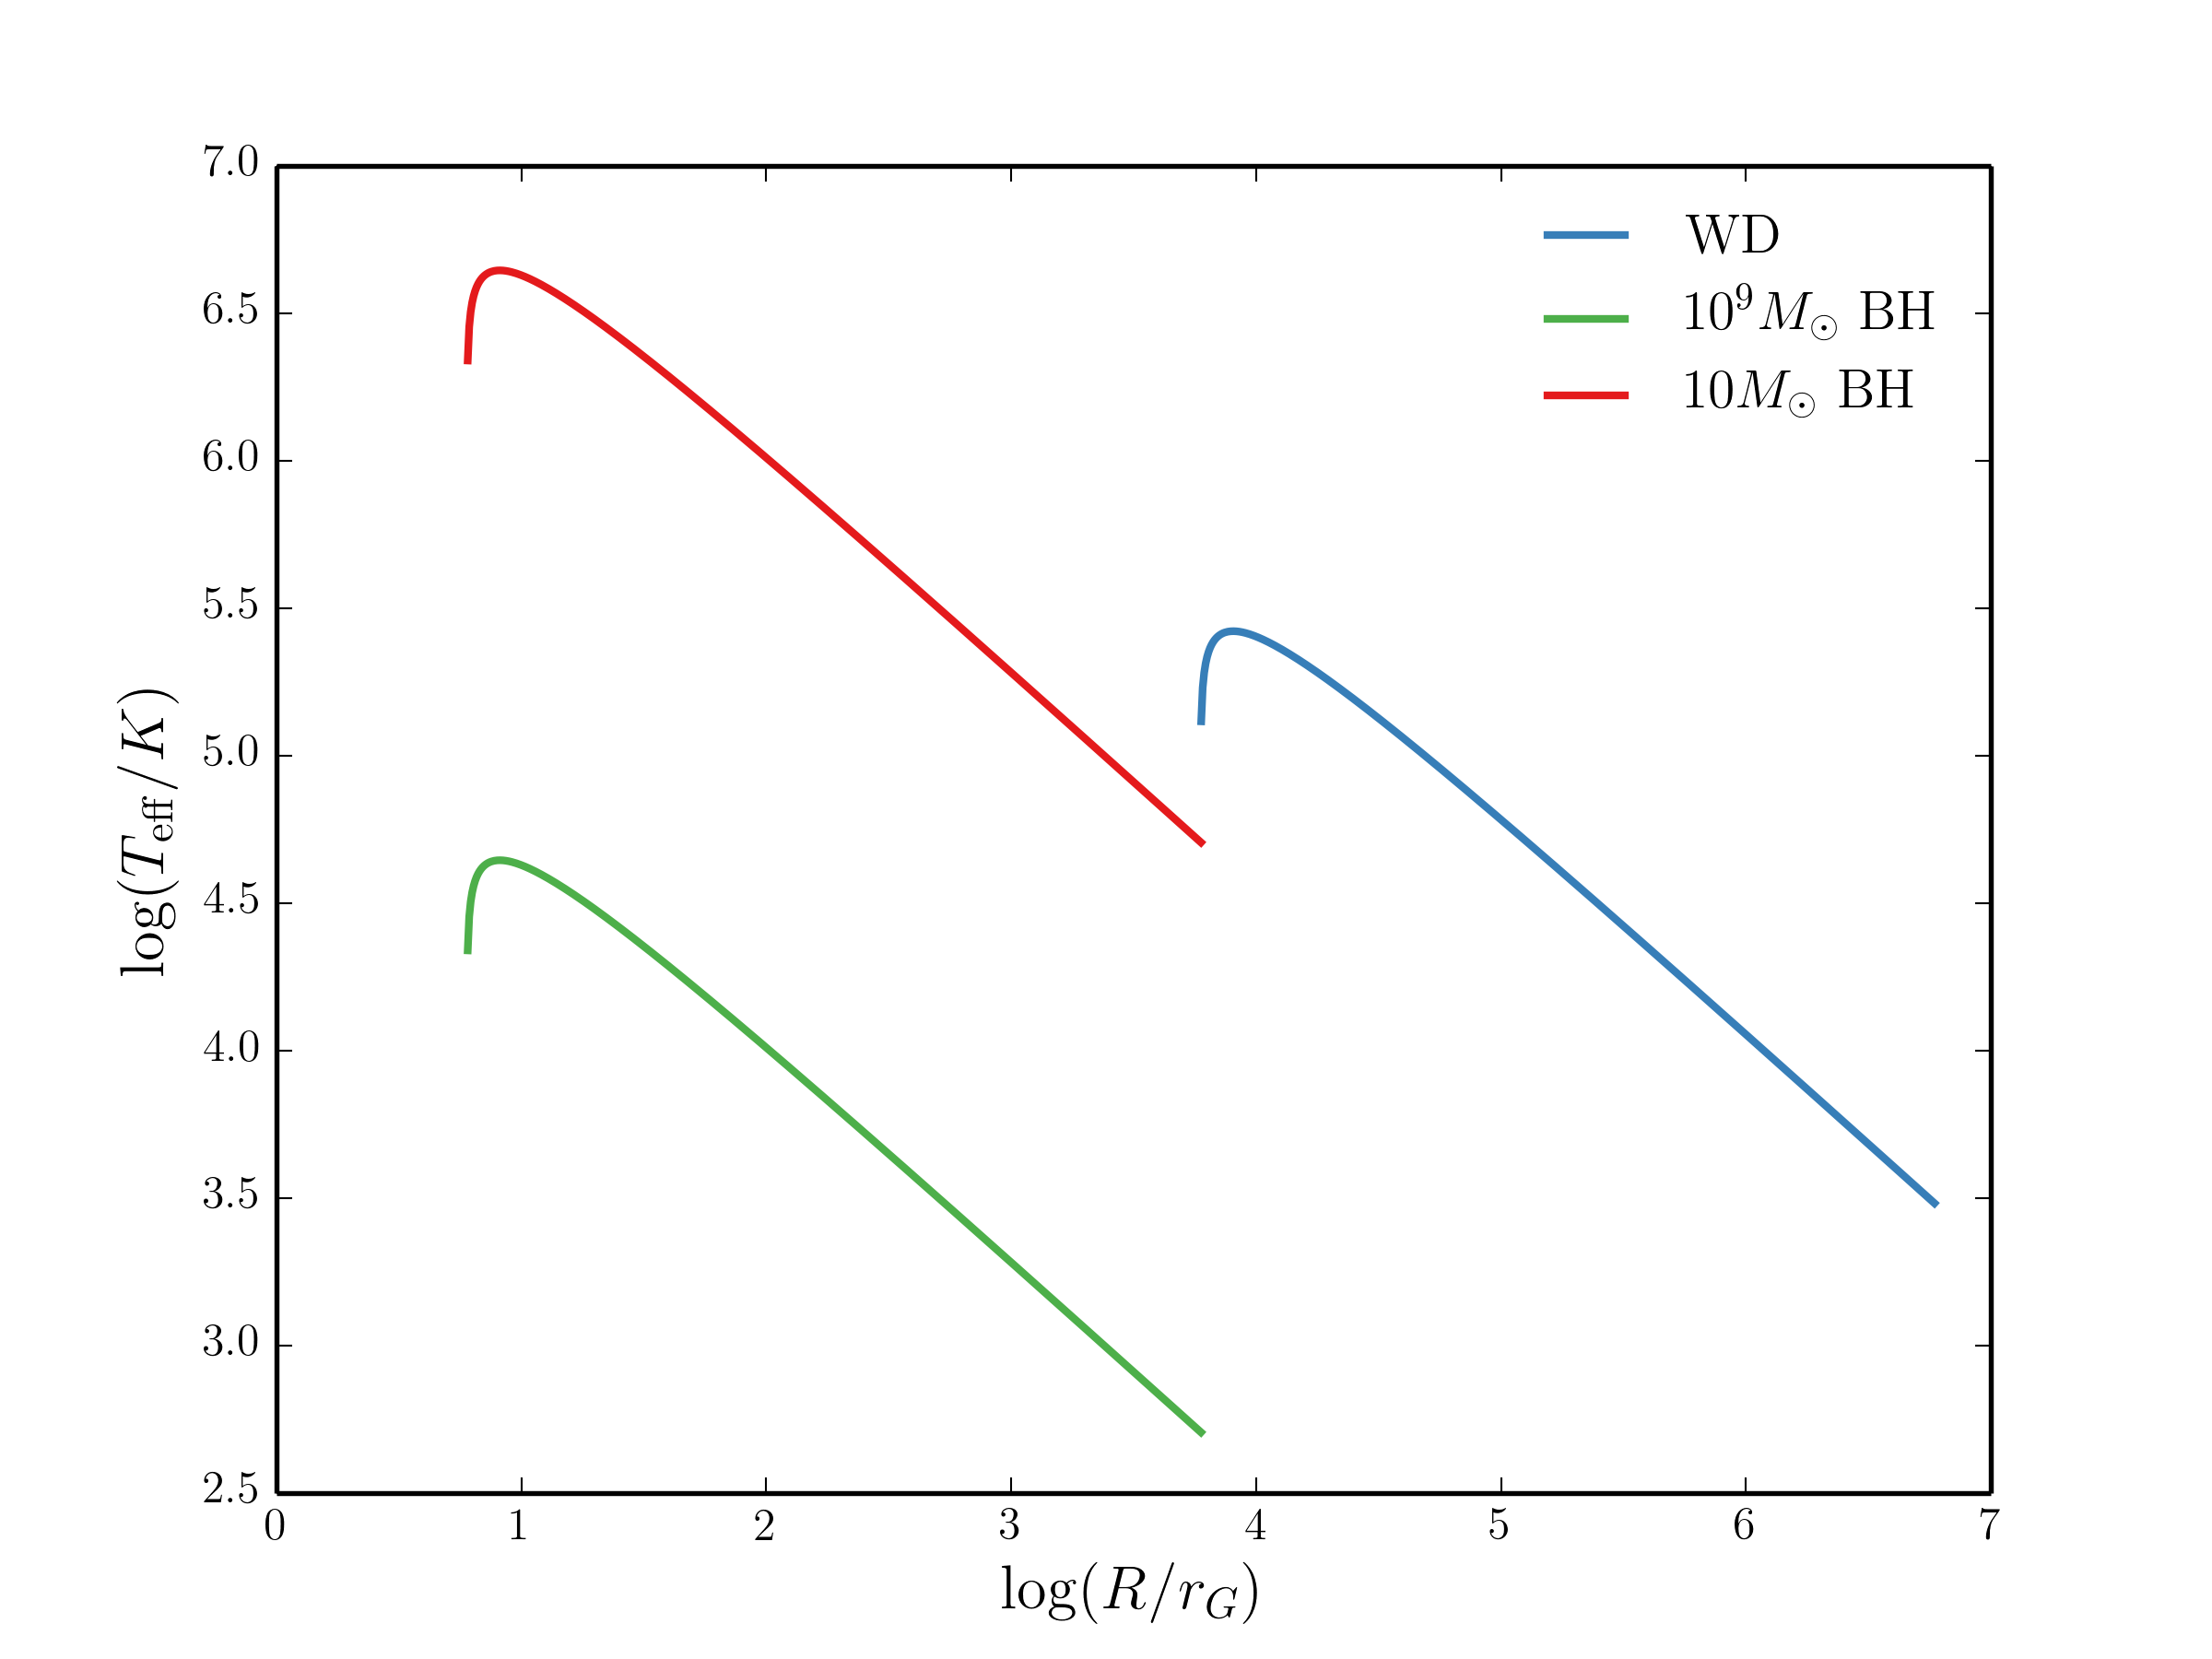
\includegraphics[width=1.0\textwidth]{figures/01-intro/disk_t.png}
\caption
[The temperature profile of an accretion disc for three different classes
of compact object.]
{
The temperature profile of an accretion disc for three different classes
of compact object.
} 
\label{fig:disk_t}
\end{figure}

It is important to recognise that the steady-state disc treatment
{\sl does not specify the nature of the disc SED}. What it does do is 
say where energy is originally released. Typically,
accretion discs are modelled as a series of annuli each emitting 
as blackbodies, but a disc atmosphere with frequency-dependent
opacity would create a somewhat different spectrum. 
Figure~? shows the blackbody SEDs expected for the same objects as figure~\ref{fig:disk_t}.
Figure~? shows a comparison between a disc atmosphere model and
blackbody model for a cataclysmic variable accretion disc, showing
the differences in spectral shape caused by frequency-dependent opacities
in the disc. It is of course possible that {\em neither} blackbody or disc atmosphere
treatments are realistic. I shall therefore devote a little time to discussing
the observational arguments for accretion discs and the different classes of accreting 
objects.


\section{Accreting Compact Binaries}

Accreting compact binaries form many different classes, 
but are all characterised by matter streaming from a donor star or secondary
onto a compact object or primary.
There are only two ways by which matter can transfer 
from the secondary to the compact object. One is by Roche Lobe-overflow (RLOF),
whereby stellar evolution causes the donor star to fill it's Roche Lobe, the surface
of equipotential around the star. The alternative is that the donor may expel
material via a disc around the secondary or radiatively driven stellar wind, 
allowing some of it to flow onto the compact object. 
Although accretion from a wind or circumstellar disc is common in 
such as high-mass X-ray binaries \citep[HMXBs; e.g.][]{bartlett2013}, here I will focus on 
RLOF as it is more common in the systems that commonly exhibit high-state accretion discs
and associated outflows.

\subsection{Roche Lobe-Overflow}

Let us consider a binary system, with masses $M_1$ and $M_2$, at positions
$\vec{r}_1$ and $\vec{r}_2$. The Roche potential, $\Phi_R$, in this system 
is then
\begin{equation}
\Phi_R = - \frac{GM_1}{| \vec{r} - \vec{r}_1 |} - 
\frac{GM_2}{| \vec{r} - \vec{r}_2 |} - 1/2 (\vec{\omega} \times
 \vec{r})^2,
\label{eq:roche}
\end{equation} 
where $\omega$ is the angular velocity of the binary and is a vector normal to
the orbital plane. This potential is plotted in figure~\ref{fig:roche} for a mass ratio, 
$q = M_2 / M_1$ of 0.25.

\begin{figure}
\centering
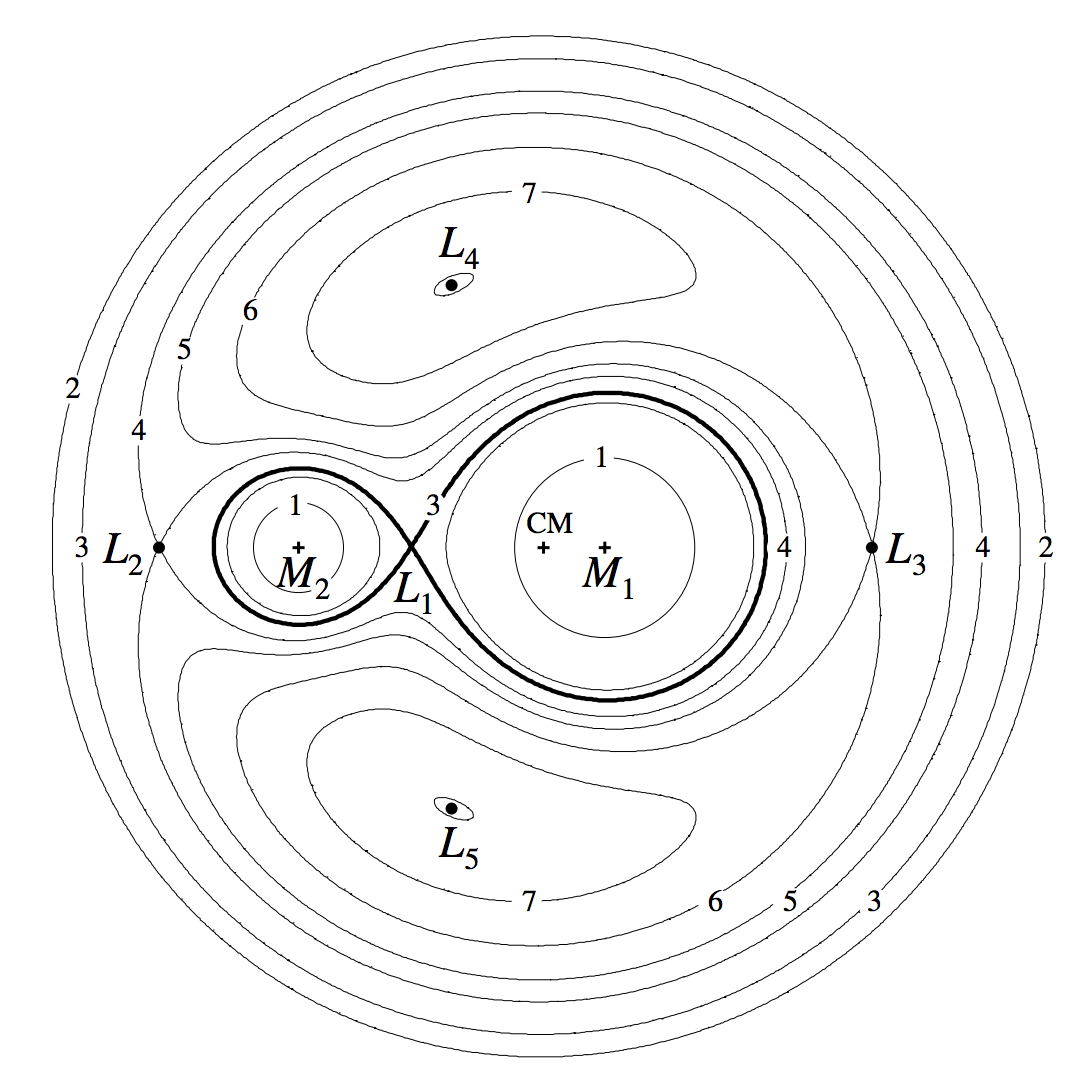
\includegraphics[width=0.7\textwidth]{figures/01-intro/roche_potential.png}
\caption
[The roche potential in a binary system]
{
{\sl Credit: Frank et al. 2002.} 
The roche potential in a binary system for $q = M_2 / M_1$ of 0.25.
The Lagrangian points are marked, as are the locations of the individual
and system centres of mass.
} 
\label{fig:roche}
\end{figure}

In the context of semi-detached binary systems, the most important region of the 
potential is the dumbbell shaped region enclosing the masses. Each of these
enclosed regions is known as the `Roche lobe' of the object and can be expressed 
approximately in terms of the mass ratio and separation of the system.
If one of the binary stars expands enough to fill its Roche lobe, then matter
will fall onto the other object. This process is known as Roche Lobe overflow (RLOF),
and is vitally important in astrophysics. Although caused by stellar evolution,
it affects the mass ratio of the binary system and thus itself affects the evolution
of binary systems. This has serious ramifications for the orbital period
distribution of binaries (REFs) as well as affecting the delay time distribution
of Type Ia Supernovae, for which CVs are one of the progenitor candidates.
It is also worth noting that the existence of gravitational waves has been 
required in models for CV evolution since 


\subsection{Cataclysmic Variables}

Cataclysmic variables (CVs) are systems in which a white dwarf
accretes matter from a donor star via Roche-lobe overflow. 
CVs are not always accreting objects; classical novae and super soft sources 
(SSS) have luminosities dominated by nuclear burning.
{\em Accreting} CVs -- the focus here -- can be classified according to the 
magnetic field strength ($B$) and photometric activity. 
Magnetic systems are classified as either `Polars' ($B \gtrsim 10^7$~G)
or `Intermediate Polars' ($10^6 \lesssim B \gtrsim 10^7$~G);
in these systems the accretion flow is dominated by the WDs 
magnetic field inside the Alfven radius (REF). In polars this radius
is large enough that no disc forms at all (REFs).
When $B \lesssim 10^6$~G then the accreting material can fall
onto the WD via a disc, and the CV is classified as non-magnetic.
There are a two main types of non-magnetic CVs; Dwarf Novae and Nova-like
variables.

\subsubsection{Nova-like Variables}

Nova-like variables (NLs) are similar to DNe in overall structure,
except that the disc is always in a relatively 
high-accretion-rate state ($\dot{M} \sim 10^{-8}$~M$_{\odot}$~yr$^{-1}$).
NLs are therefore one of the best `laboratories' for testing the steady-state
accretion disc theory described in section~\ref{sec:alpha_disc}.
NLs generally exhibit a series of strong emission lines superposed on a 
blue continuum. 

\nocite{dhillon1996,hessman1984}
\begin{figure}
\centering
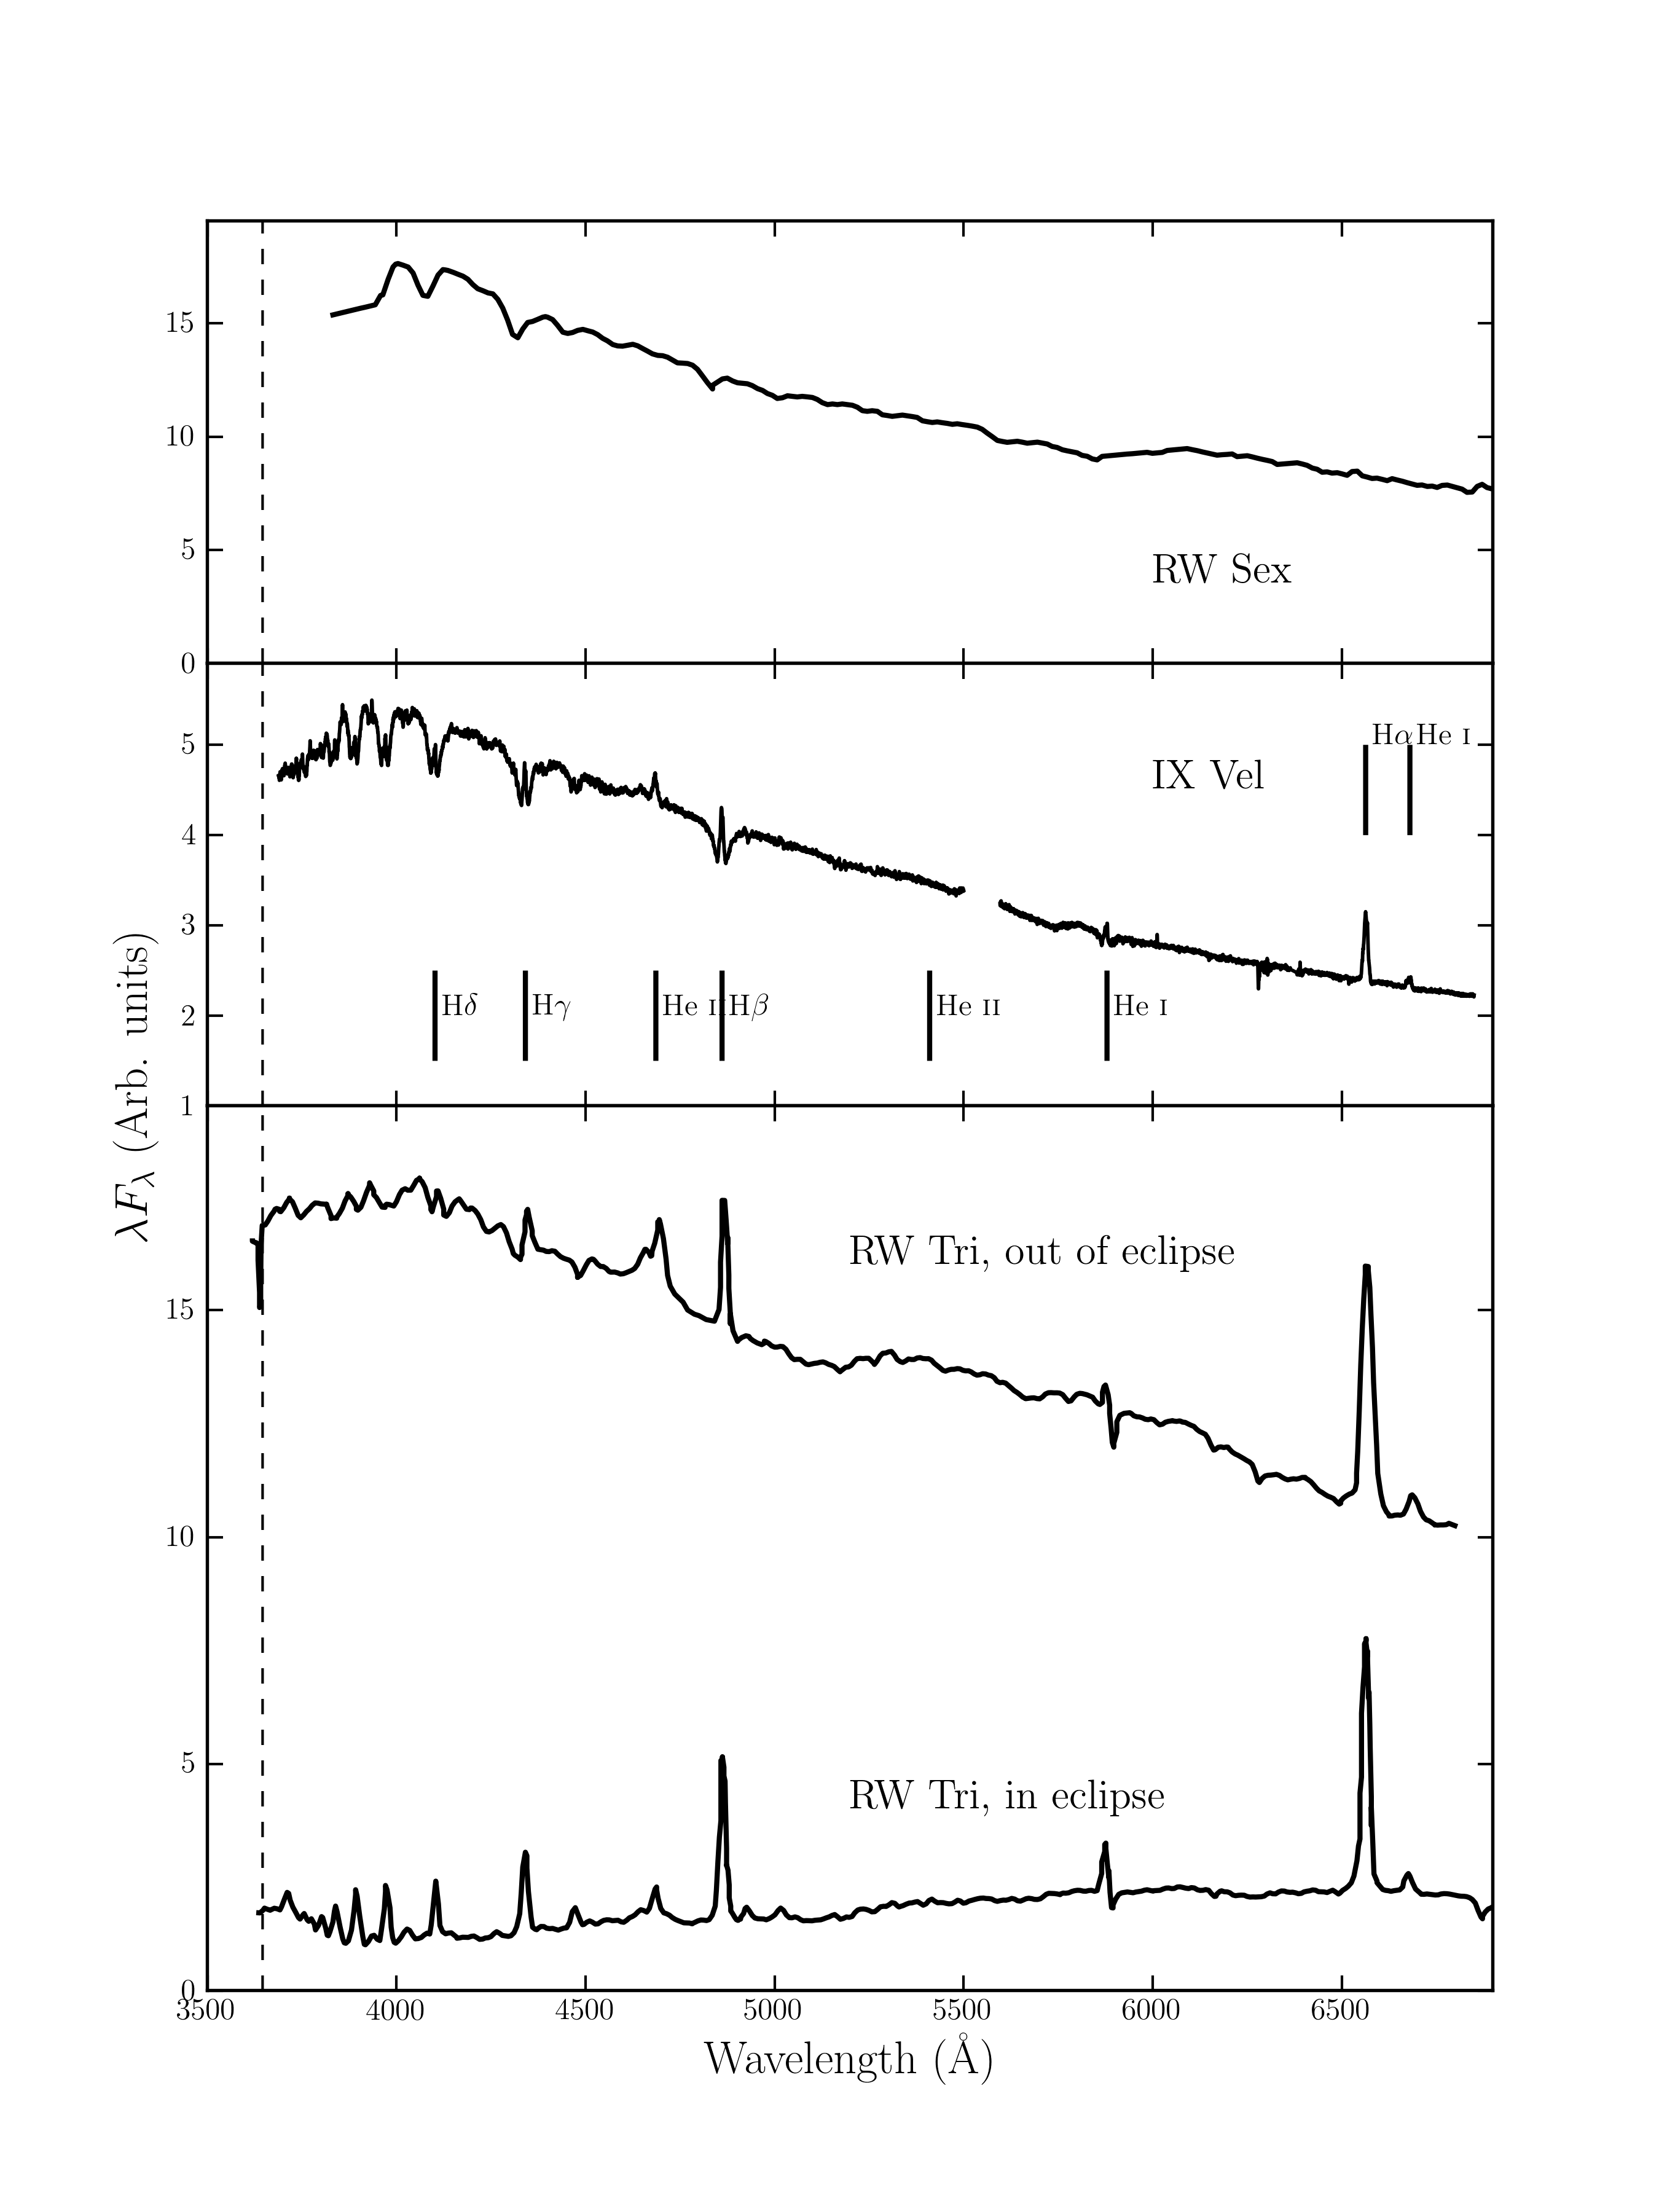
\includegraphics[width=1.0\textwidth]{figures/01-intro/novalikes.png}
\caption
[Optical spectra of three nova-like variables.]
{
Optical spectra of three nova-like variables.
} 
\label{fig:kording_hid}
\end{figure}


\subsubsection{Dwarf Novae and the Disc-instability Model}

Dwarf novae (DNe) are accreting systems that are characterised 
by periods of quiescence and outburst on varying timescales. One of the 
most famous DNe is SS Cyg, whose century of activity is shown in 
figure~\ref{fig:sscyg}. The repeated outbursts, with characteristic 
shape, can be clearly seen.

\nocite{dhillon1996,hessman1984}
\begin{figure}
\centering
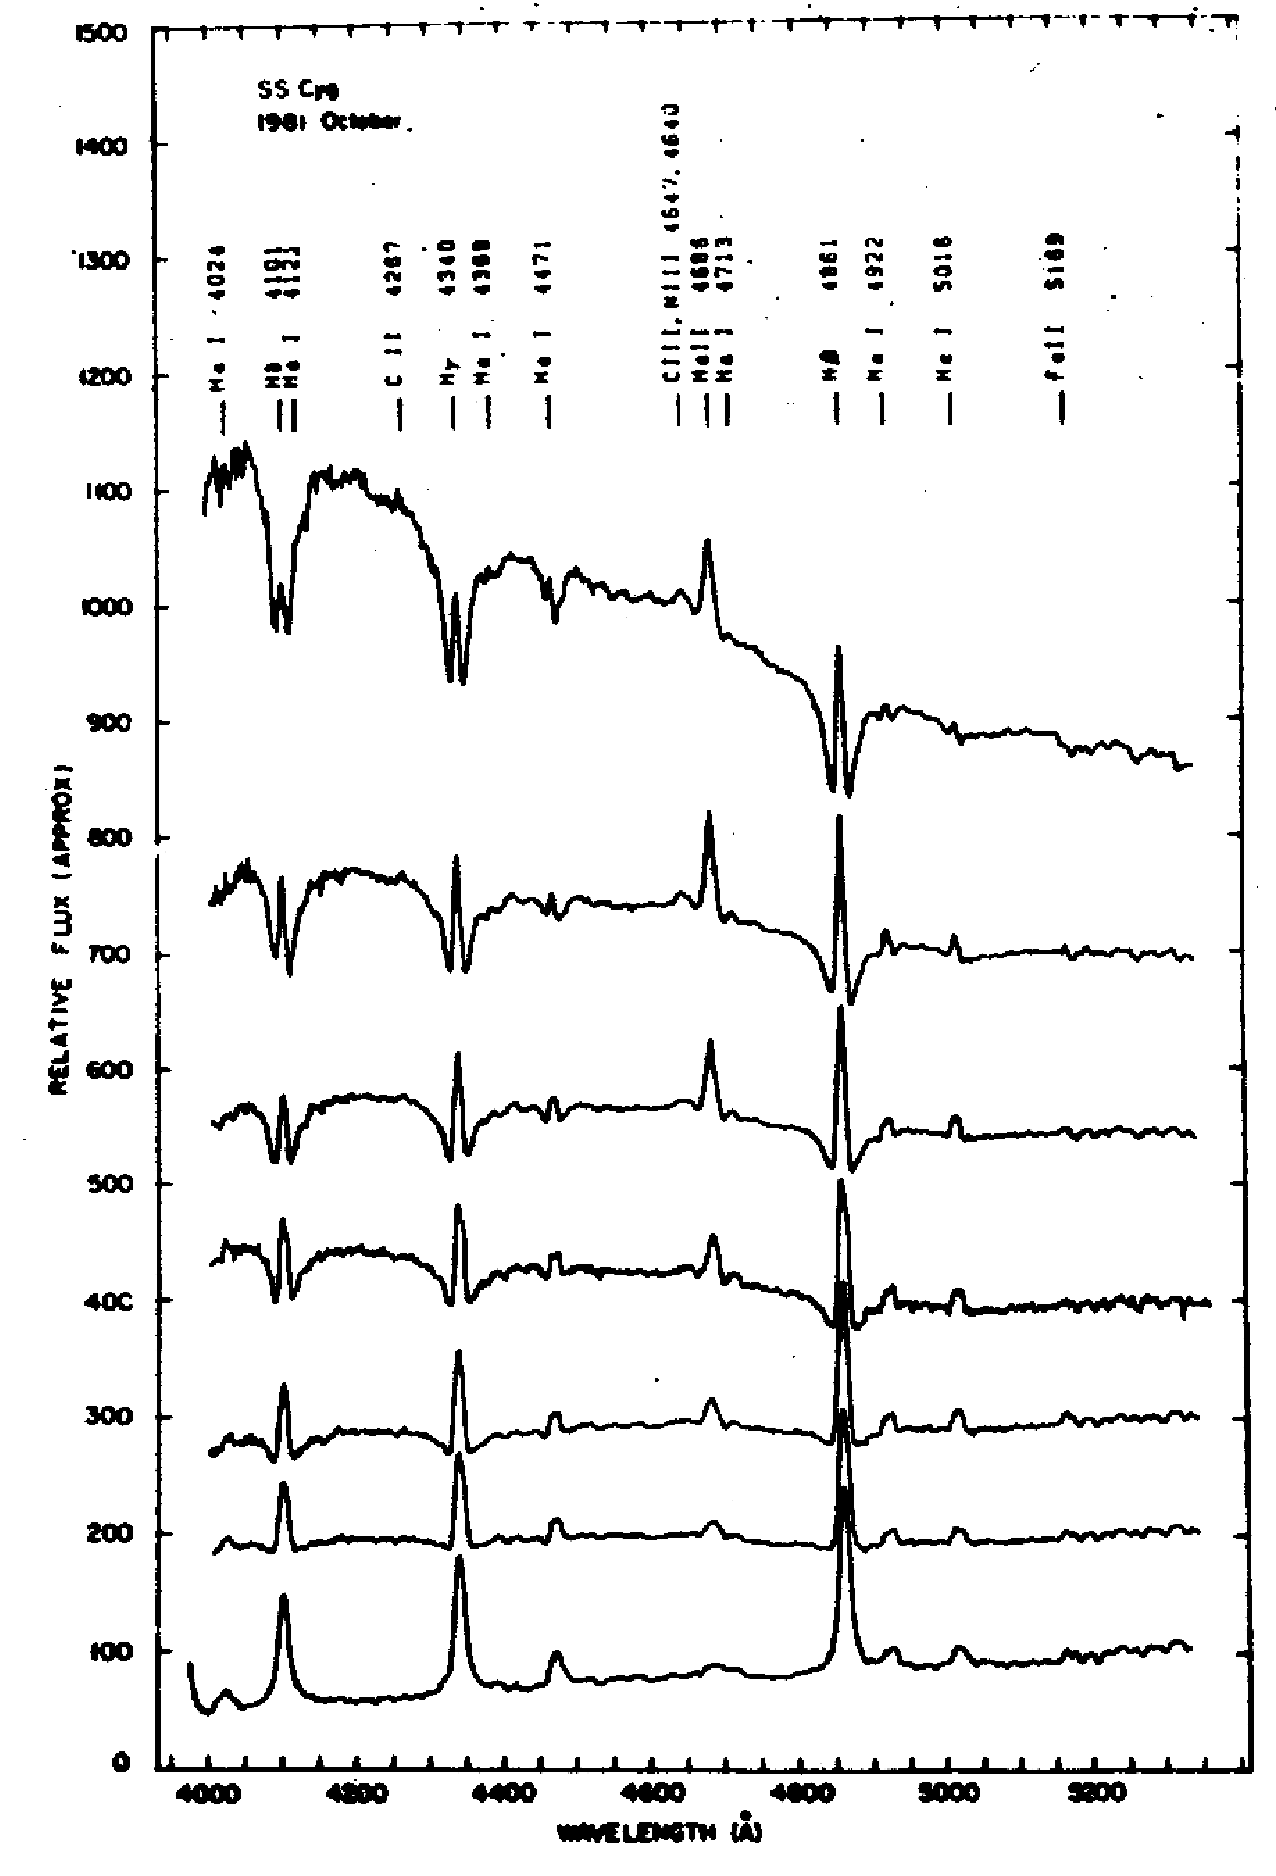
\includegraphics[width=1.0\textwidth]{figures/01-intro/sscyg_spec.png}
\caption
[Spectra of SS Cyg during an outburst cycle]
{
{\sl Credit: Hessman et al. 1984 / Dhillon et al. 1996.} 
Spectra of SS Cyg during an outburst cycle, showing the evolution from 
minimum to maximum light. The rise is characterised by the appearance of an
optically thick accretion disc spectrum. The flux scale is approximate.
} 
\label{fig:kording_hid}
\end{figure}


\subsection{Low Mass X-ray Binaries}

X-ray binaries are similar to CVs in structure, except that the compact object
is either a neutron star (NS) or black hole (BH). The accretion disc 
emits in the soft X-rays, and an additional hard X-ray power law is also 
seen in the spectrum (REFs). This hard component is normally attributed
to Compton up-scattering of seed disc photons by some kind of `corona'
of hot electrons close to the BH (REFs). A characteristic spectrum is shown 
in figure~\ref{fig:xrb_spec}.

Although I do not discuss XRBs directly in this thesis, it is instructive
to discuss some of their observational appearance as it is instructive 
for understanding the theory of disc winds, as well as their wider significance. 
The discovery that XRBs follow similar tracks on a hardness-intensity diagram (REFs)
is particularly interesting in this regard, especially since \cite{ponti2012}
showed that broad Fe absorption lines are only seen in the soft-state 
high-inclination systems (see section~\ref{sec:xrb_winds}). 
This implies that equatorial outflows are intrinsic to 
the accretion process. Although the driving mechanism
is almost certainly different to CVs (REFs), the similarity in general structure 
to models for CVs and quasars is striking.


% \begin{figure}
% \centering
% 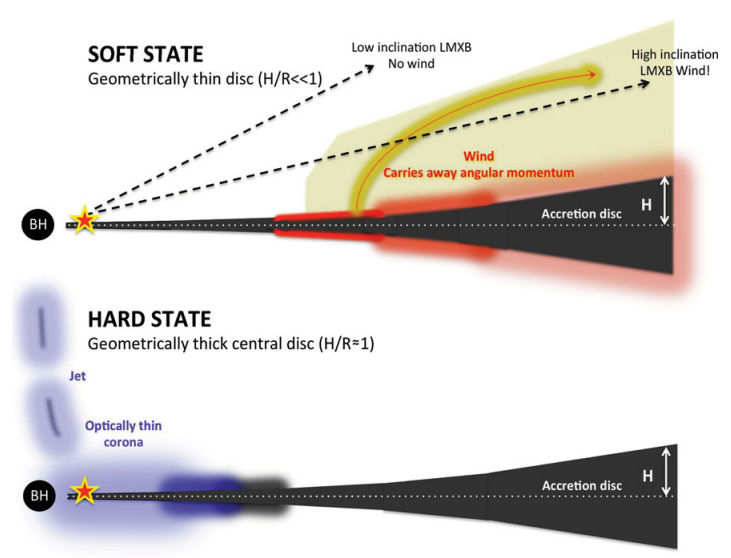
\includegraphics[width=0.7\textwidth]{figures/01-intro/ponti_wind_cartoon.png}
% \caption
% [Hardness intensity diagram for a WD, NS and BH system]
% {
% {\sl Credit: Ponti et al. 2012}
% Hardness intensity diagram for a WD, NS and BH system
% } 
% \label{fig:ponti_cartoon}
% \end{figure}


\section{Quasars and Active Galactic Nuclei}

Spectra of AGN have now been studied for over 100 years, and we have known 
that they exhibit strong, broad emission lines since the first spectrum was taken by
\cite{fath1909}.
However, it wasn't until the work of \cite{seyfert1943} that the systematic 
classification of AGN really began, leading to the phrase `Seyfert galaxy'.
This label was applied to galaxies possessing a bright nucleus, spectroscopically
characterised by a blue continuum and a series of strong emission lines.
The first real physical insight into the extraordinary nature of AGN
was provided by \cite{woltjer1959}, who noted that (i) the nuclei must have sizes $<100$~pc,
based on the fact that they were unresolved and (ii) the mass of the nucleus
must be very high, based on virialised motion. 
While both of these observations were based on simple arguments, the fact that these
ultra-luminous celestial objects are both {\em compact} and {\em supermassive}
is perhaps the defining insight into the nature of AGN.

Although the field of AGN study was established in the optical, 
radio astronomy also significantly furthered our understanding of AGN
in the mid-20th century. A number of surveys, such as the Cambridge \citep{edge1959}, 
Parkes \citep{ekers1969} and Ohio \citep{ehman1970} surveys discovered a great many 
bright radio point sources distributed isotropically across the sky.
These sources eventually became known as `quasi-stellar radio sources'
or {\em quasars}, and were soon identified to be coincident with bright optical
sources or `quasi-stellar objects' (QSOs; REFs). 
Nowadays, the term quasar normally has very little to do with 
radio emission and is often used interchangeably with QSO. 
Indeed, throughout this thesis I shall refer to a quasar as simply a bright, 
massive AGN; one with sufficiently high luminosity that it dominates the emission 
from it's host galaxy.

\subsection{AGN Taxonomy}
\label{sec:agn_taxonomy}

In addition to Seyfert galaxies and quasars, there are a number of 
different classes of AGN. These are broadly characterised by their spectra in the 
optical, UV and X-ray as well as their radio behaviour. It is worth noting
that these are observational classifications; that is, even after a century
of study, the {\em physical} origins of the diverse behaviour of AGN
are still an active area of research.

\begin{figure}
\centering
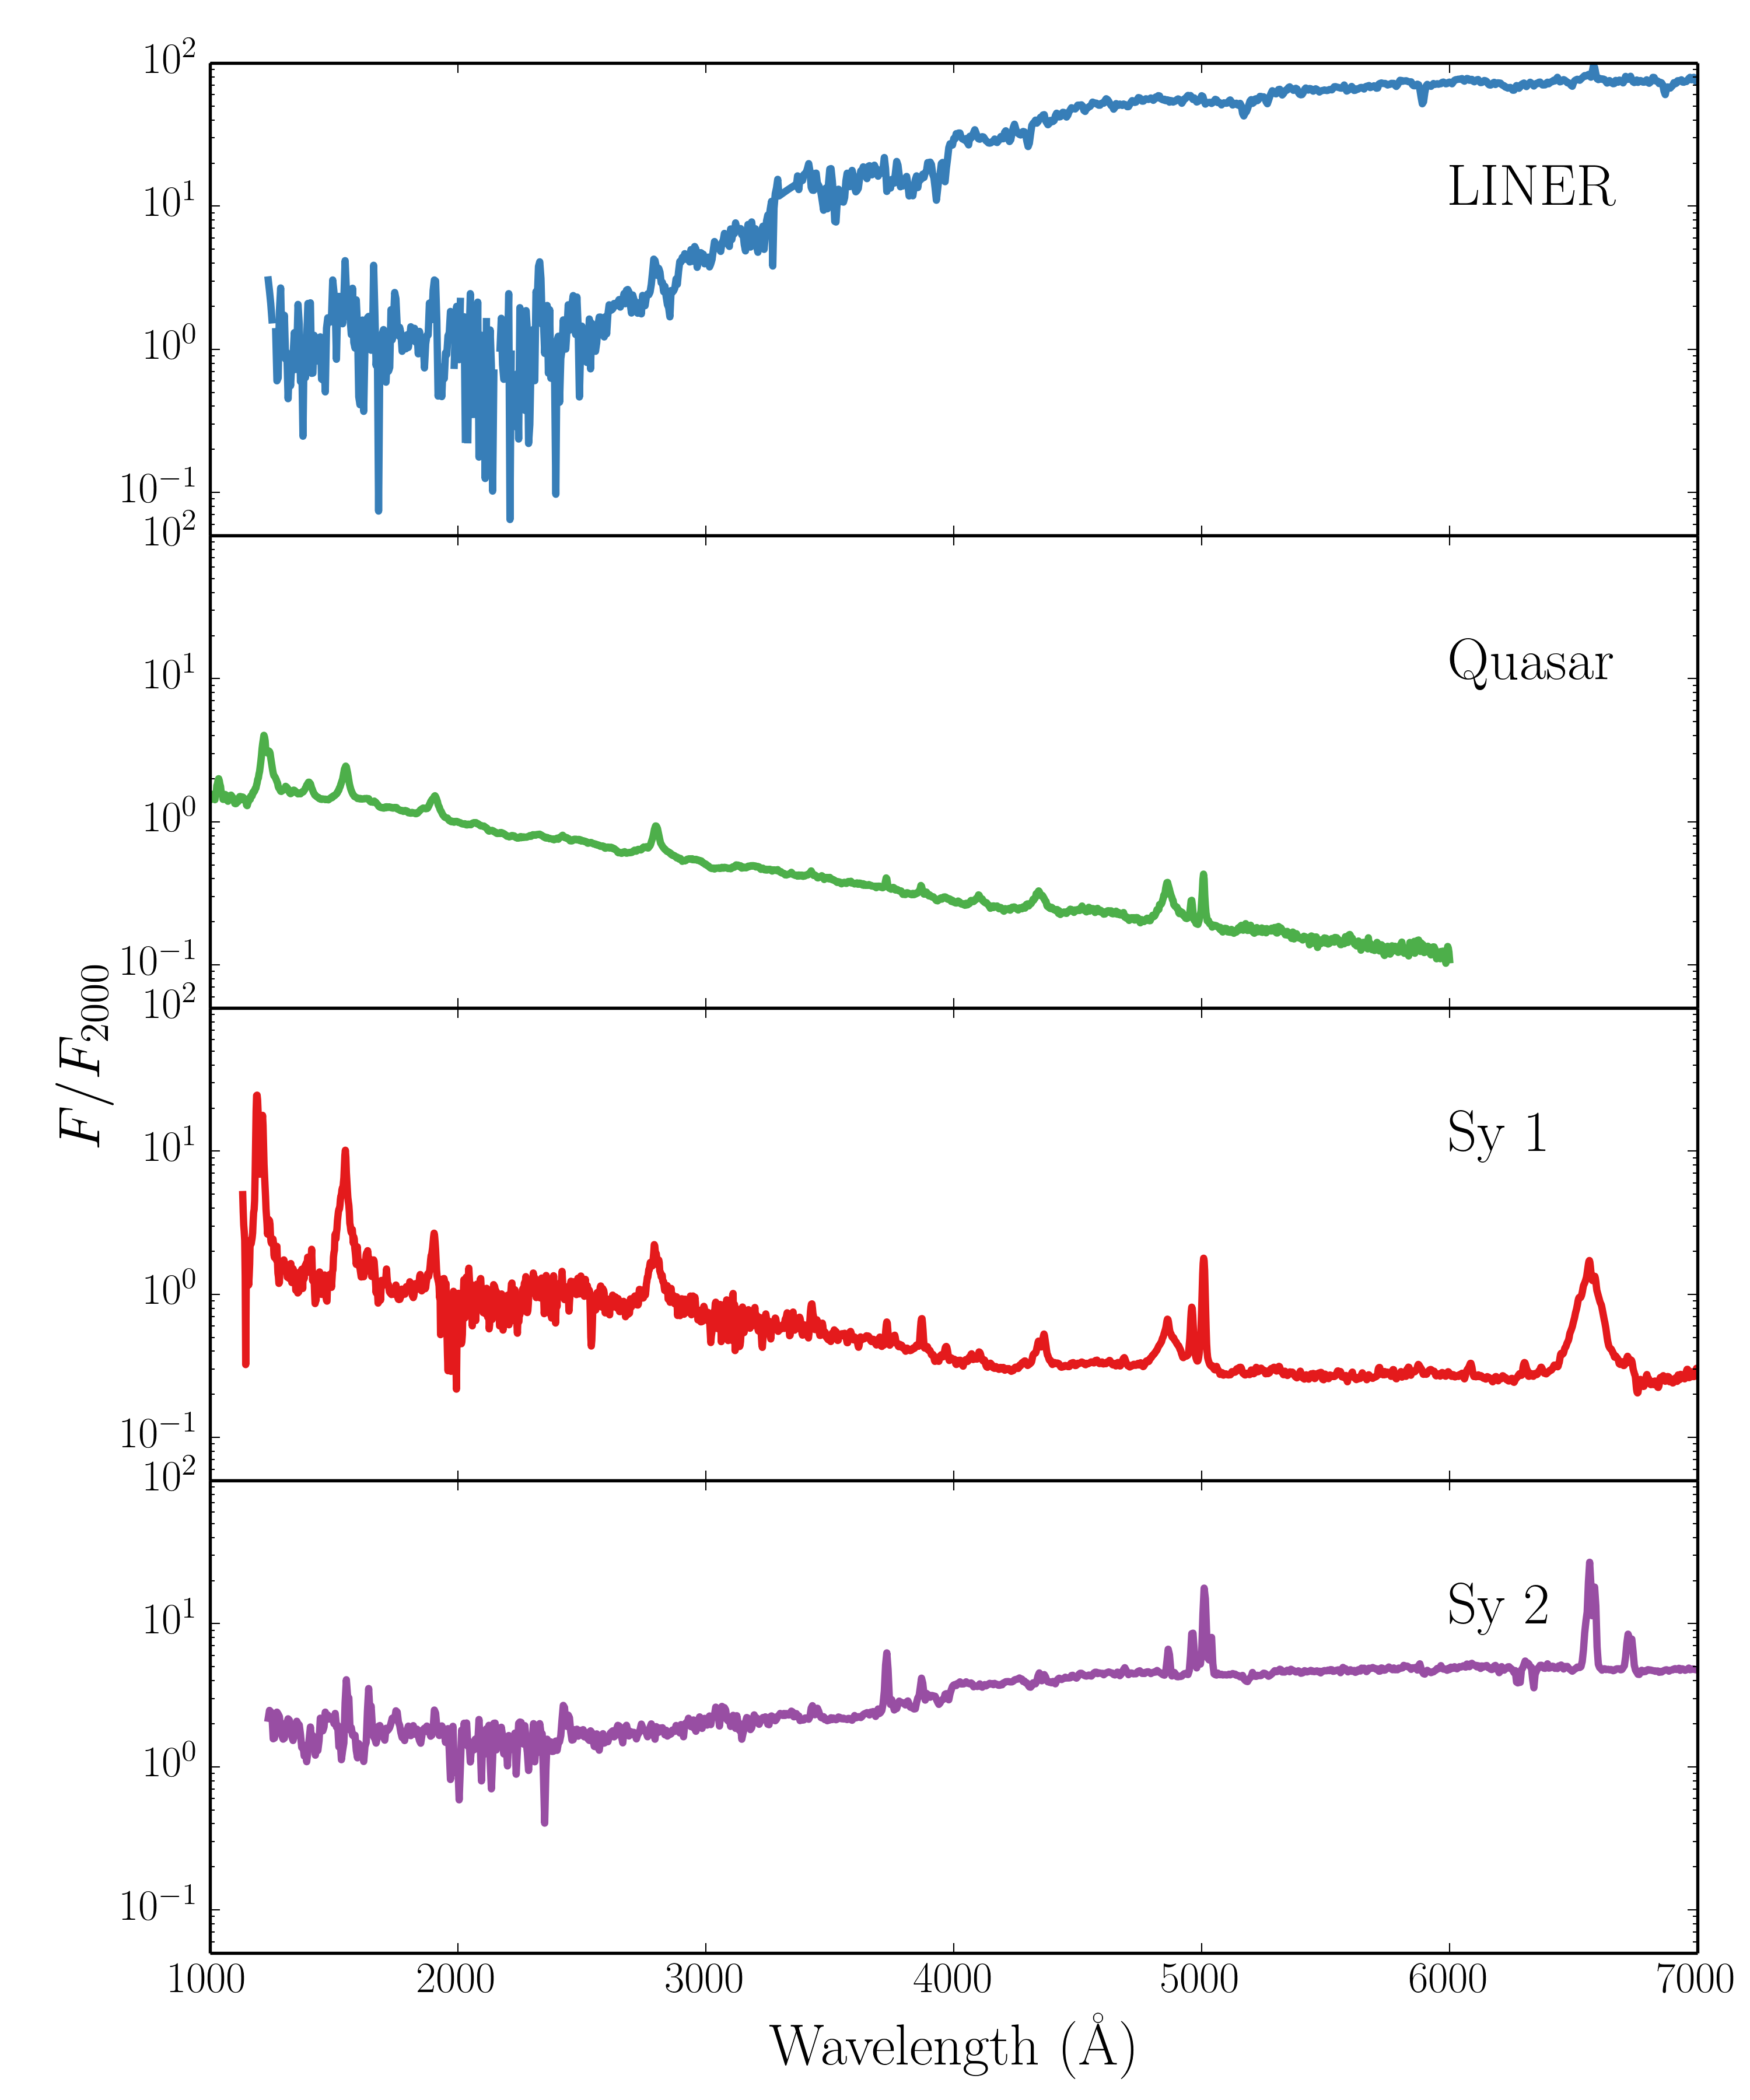
\includegraphics[width=1.0\textwidth]{figures/01-intro/agn_templates.png}
\caption
[Template spectra, from the AGN atlas, for four common types of AGN.]
{
Template spectra, from the AGN atlas, for four common types of AGN.
Obtained from \url{http://www.stsci.edu/hst/observatory/crds/cdbs_agn.html}.
} 
\label{fig:agn_templates}
\end{figure} 

\subsubsection{Radio Galaxies}

\subsubsection{BL Lacs and Blazars}

BL Lac objects -- named for the first object of the class, BL Lacertae --
are AGN with featureless non-thermal continua (REFs), in contrast to Seyfert
galaxies. Their optical flux is highly polarised (REFs) and they tend to
exhibit large-scale optical variability (REFs). BL Lacs are a subset of 
a larger AGN class known as Blazars, the most luminous of which
are known as optically violent variable (OVV) quasars. 
Blazars require relativistic beaming in order to explain their high 
radio luminosities (REFs), implying that the jet is orientated towards
the observer (REFs). These objects thus have an important place in unification
schemes (see section~\ref{agn_unification}), and also 
allow us to learn directly about the Lorentz factors and shock physics
of relativistic radio jets (REFs).

\subsubsection{LINERs}

\subsubsection{Low-luminosity AGN}


\subsection{AGN Unification and the dusty Torus}
\label{agn_unification}

Although Seyfert had identified type 1 and 2 AGN, a physical explanation
for this dichotomy was not forthcoming until a study by \cite[][AM85]{antonucci1985}.
They showed unambiguously that the nearby Seyfert 2 NGC~1068 is simply an obscured
type 1 AGN, by finding that broad emission lines appeared in the spectrum of
{\em polarised} flux. This provided the basis for the first successful attempt
to unify AGN behaviour, as it elegantly 
explained the apparent disconnect between the two types of 
AGN as simply a viewing angle effect. 
The obscuring structure became known as the `torus' \citep{krolik1986}, 
due to its geometry, and it was soon realised that this structure
may be made of dust, in which case it could also be responsible for the infra-red (IR)
bump in AGN \citep{neugebauer1979}.

The \citep[][UP95]{UP95} scheme went further than the original unification model
proposed by AM85 as it also attempted to explain radio AGN phenomena.
The picture they proposed is shown in figure~\ref{fig:unification}.
This model attempts to explain all of the types of AGN described in
section~\ref{sec:agn_taxonomy} merely as a function of viewing angle
and presence, or lack thereof, of a radio jet.

\begin{figure}
\centering
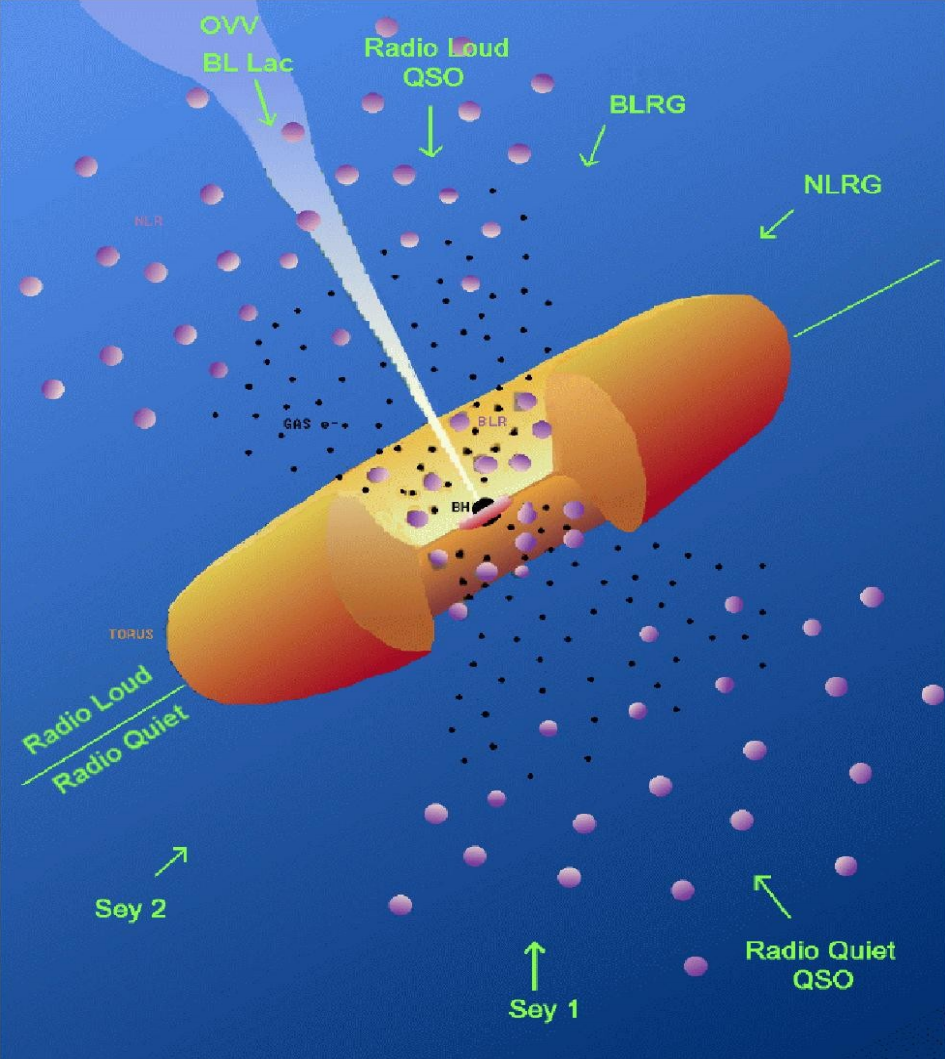
\includegraphics[width=1.0\textwidth]{figures/01-intro/up95.png}
\caption
[A unified scheme for AGN.]
{
A unified scheme for AGN.
} 
\label{fig:unification}
\end{figure} 

Since the seminal works by AM85 and UP95, 
the picture has become somewhat more complicated. 
Variable X-ray absorption has been detected in so-called `Changing look'
AGN \citep{matt2003,puccetti2007}, even in NGC 1068 itself \citep{marinucci2016}.
Changes in type have also been seen in the optical lines; 
the broad H$\beta$ component can dramatically disappear or reappear
\citep[e.g.][]{tohline1976,cohen1986,denney2014}. 
The explanation for this could be variable absorption \citep{elitzur2012}
or linked to the accretion state of the disc. In the latter case,
it has even been suggested that a disc wind could be directly responsible
for this change in accretion state \citep{elitzur2014}.
Furthermore, dusty {\em polar} outflows
have been found to be important IR emitters \citep{hoenig2013}, implying
that, even when it comes to dust, the torus is not the whole picture.
Despite these complications, the AGN torus unification picture still helps 
explain a lot of AGN behaviour, and represents a good framework 
to test with observations. 

\subsection{The Broad Line Region and Connection to Outflows}

In the UP95 unification model, the broad emission lines
come from a series of virialised clouds close to the disc plane.
As noted by \cite[][hereafter MCGV95]{MCGV95}, there are a number of problems with
the BLR `cloud' model, perhaps most notably that there is no obvious 
physical origin for a series of virialised clouds. While there are exceptions
to this statement (REFs), it is important to test other models.
Indeed, MCGV95 proposed a disc wind model in order to explain both BALs and BELs
in quasars. A disc wind model was also  discussed by \cite{elvis2000}, 
who proposed a structure for quasars that attempted to explain much 
of the behaviour of luminous AGN
merely as a function of viewing angle. Outflow models are discussed further in section~2.
The philosophy of these models is that, before invoking additional
degrees of freedom in a model, we should first test if known quasar phenomenology 
(winds) can explain other aspects of their observational appearance.
I have illustrated this general principle with the `Occam's quasar' 
cartoon shown in figure~\ref{fig:occam}. This is the picture that I will
quantitatively test in the latter, quasar-focused sections of this thesis, and the general
principle can even be applied to cataclysmic variables and other accreting objects.


\begin{figure}
\centering
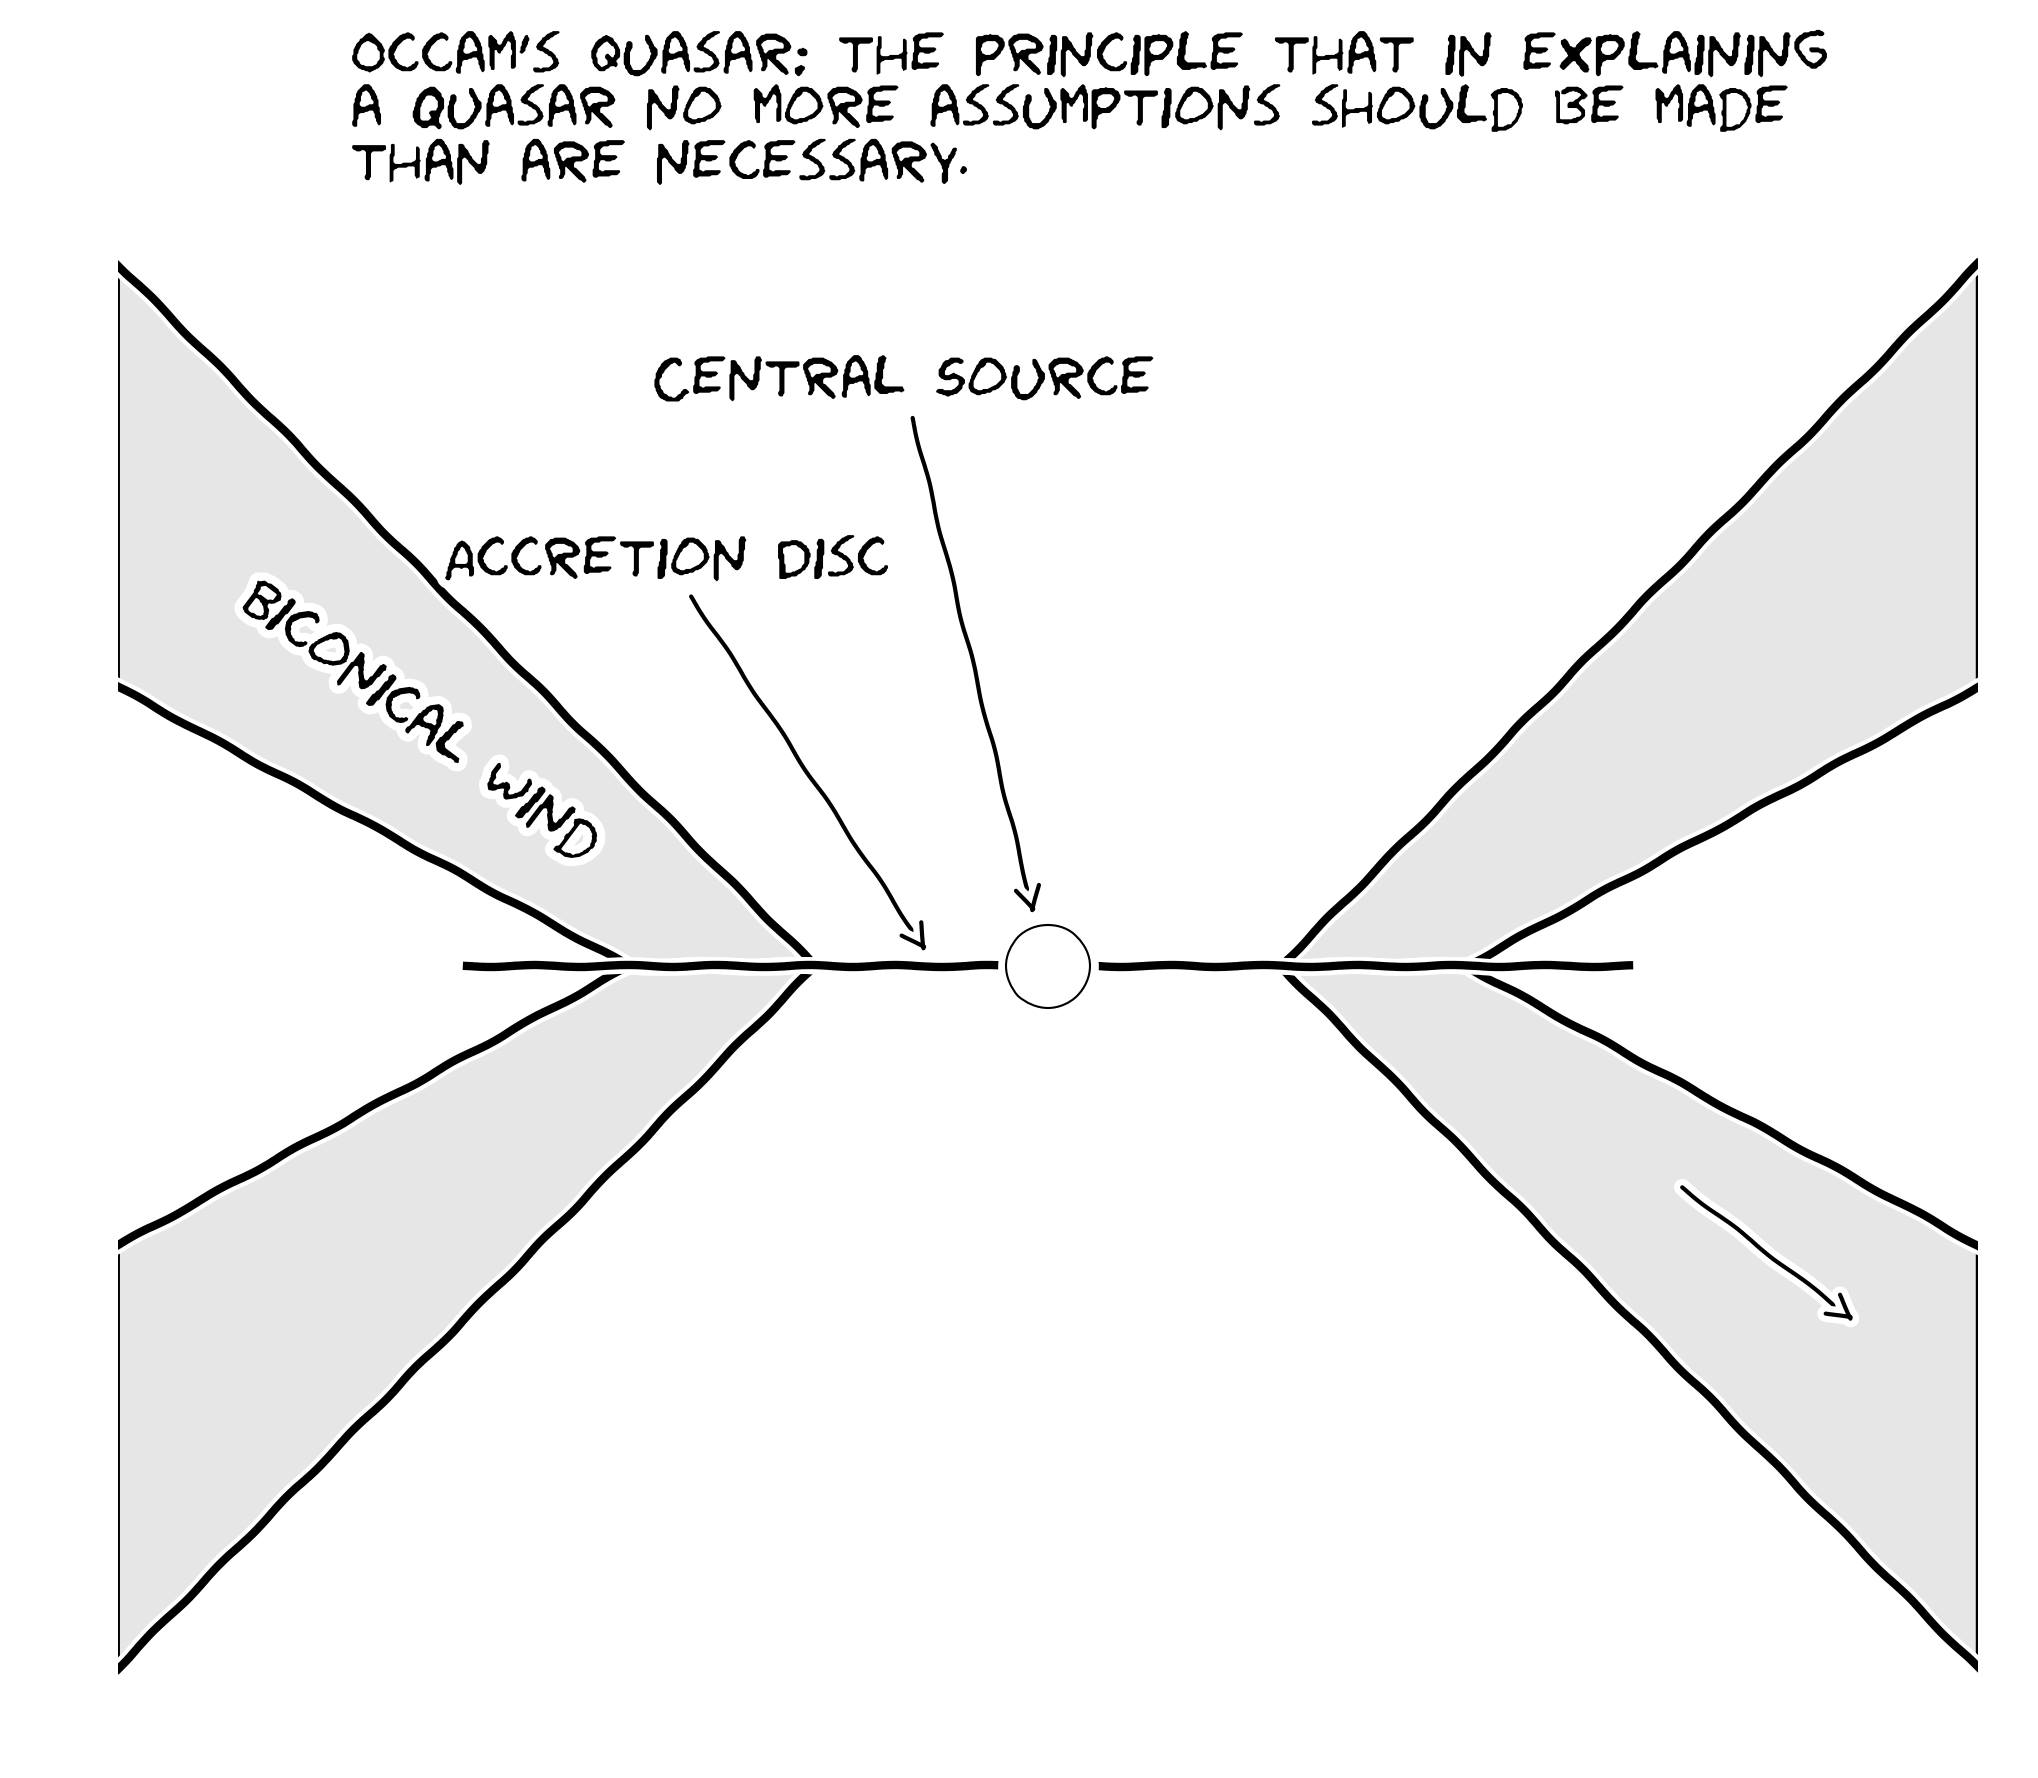
\includegraphics[width=1.0\textwidth]{figures/01-intro/occam.jpg}
\caption
[Occam's quasar]
{
Occam's quasar. How far can this general picture take us when trying to explain
the behaviour of quasars and other accreting compact objects?
} 
\label{fig:occam}
\end{figure}


\section{The Current Understanding of the Disc Continuum}

A number of issues have been raised with the thin-disc model and
its applicability to accreting systems. 

\subsection{The Spectral shape of CV discs}

Attempts to fit the observed SEDs of high-state CVs with simple disc models 
have met with mixed success. In
particular, the SEDs predicted by most stellar/disc atmosphere models 
are too blue in the UV \citep{wade1988,long1991,long1994,knigge1998} and exhibit
stronger-than-observed Balmer jumps in absorption 
\citep{wade1984,haug1987,ladous1989b,knigge1998}. One possible
explanation for these problems is that these models fail to capture
all of the relevant physics. Indeed, it has been argued that a
self-consistent treatment can produce better agreement with 
observational data (e.g. Shaviv et al. 1991;  but see also Idan et al. 2010).
\nocite{idanshaviv2010} \nocite{shaviv1991}
However, an alternative explanation, suggested by Knigge et al.
(1998b; see also Hassall et al. 1985)\nocite{KLWB98,hassall}, 
is that recombination continuum emission from the base of the 
disc wind might fill in the disc's Balmer absorption edge and flatten the UV spectrum.

\subsection{The Big Blue Bump in AGN}

\subsubsection{The Accretion Disc Size Problem}

One of the most interesting results of recent years relating to AGN and accretion discs is
the discovery that the continuum emission region size is a factor $\sim3$ larger than
predicted by standard Shakura \& Sunyaev disc theory. This result
has been found independently in both microlensing \citep{morgan2010} 
and reverberation \citep{edelson2015}. 

\subsubsection{The Soft-Xray Excess}


\section{The Universality of Accretion}

Accretion appears to be an important physical processes across $\sim10$ orders
of magnitude in mass. But is this process the same at all scales? Does any 
behaviour manifest in all accretion systems? 

\subsection{The RMS-flux relation}

Broad-band variability is common in all types of accretion disc. It has been
known for some time that there exists a linear relationship
between the flux and absolute root-mean-square (rms) amplitude
of this variability. This was discovered first in XRBs and AGN 
\citep{uttley2001, uttley2005, heil2012}, but it has been shown
more recently that the relationship extends to CVs and even YSOs 
\citep{scaringi2012,scaringi2015a}. The relationship is not limited
to one type of CV, as it is present in both NLs and DNe \citep{vandesande2015}.
 
The model that best reproduces this behaviour is the so-called
`fluctuating accretion disc' model \citep{lyubarskii1997,kotov2001,
arevalo2006,hogg2015}. It has been shown that 
additive processes cannot reproduce the behaviour, and a multiplicative
mechanism is required \citep{uttley2005}. 
Regardless of the mechanism, the rms-flux relation is one of the most
clear-cut examples of a universal accretion phenomenon. 
It tells us that at least some of the behaviour in CV discs
is present in AGN and XRBs, strengthening the argument that CVs
should be used as `accretion laboratories'. 


\subsection{Accretion States}


\begin{figure}
\centering
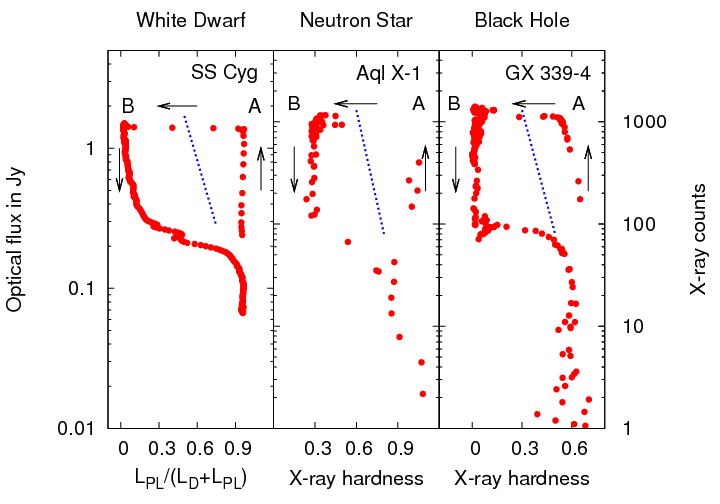
\includegraphics[width=0.7\textwidth]{figures/01-intro/kording_hid.png}
\caption
[Hardness-intensity diagrams for three types of accreting objects.]
{
{\sl Credit: Kording et al. XXXX.} 
Caption.
} 
\label{fig:kording_hid}
\end{figure}



\subsection{Jets and Outflows}


\subsection{A Global Picture}

Clearly, accretion physics is relevant to a plethora of astrophysical phenomena. 
It would also appear that the outflowing material observed in accreting systems 
has a profound effect on the accretion process itself, as well as acting 
as a spectral `filter' -- modifying, and sometimes dominating the observational 
appearance of accretion discs.

